\subsection{Adaptive Loop Construction}

Although mesh-based PDE 
codes are capable of providing results to the required levels of
accuracy, the vast majority lack the ability to automatically control
the mesh discretization errors through the application of adaptive
methods \cite{AiOd00,BaSt01,BaRa03}, thus leaving it to the user to
attempt to define an appropriate mesh.

One approach to support the application of adaptive analysis is to
alter the analysis code to include the error estimation and mesh
adaptation methods needed. The advantage of this approach is that the
resulting code can minimize the total computation and data
manipulation time required. The disadvantage is the amount of code
modification and development required to support mesh adaptation
is extensive since it requires extending the data structures
and all the procedures that interact with them. The expense and time
required to do this for existing fixed mesh codes is large and, in most
cases, considered prohibitive.

The alternative approach is to leave the fixed mesh analysis code
unaltered and to use the interoperable mesh, geometry and field
components to control the flow of information between the analysis
code and a set of other needed components. This approach has been used
to develop multiple adaptive analysis capabilities in which the
mesh, geometry and field components are used as follows.

\begin{itemize}
\item The geometry interface supports the integration with multiple
CAD systems. The API of the modeler enables interactions
with mesh generation and mesh modification to obtain all domain
geometry information needed \cite{BeWa04}.

\item The mesh interface provides the services for storing and
modifying mesh data during the adaptive process. The
Algorithm-Oriented Mesh Database \cite{ReSh03} was used for the examples given
here.

\item The field interface \cite{BeSh99} provides the functions to obtain
the solution information needed for error estimation and to support
the transfer of solution fields as the mesh is adapted.
\end{itemize}

One approach to support mesh adaptation is to use error estimators
to define a new mesh size field that is provided to an
automatic mesh generator that creates an entirely new mesh
of the domain. Although a popular approach, it has two
disadvantages. The first is the computational cost of an entire mesh
generation each time the mesh is adapted. The second is that in the
case of transient and/or non-linear problems, it requires global
solution field transfer between the old and new meshes. Such solution
transfer is not only computationally expensive, it can introduce
additional error into the solution which can dictate the ability of
the procedure to effectively obtain the level of solution accuracy
desired. An alternative approach to mesh adaptation is to apply local
mesh modifications \cite{LiSh05} that can range from standard templates, to
combinations of mesh modifications, to localized remeshing. Such
procedures have been developed that ensure the mesh's approximation to
the geometry is maintained as the mesh is modified \cite{LiSh03}. This is the
approach used to adapt the mesh in the examples presented here.

\subsubsection{Adaptive Loop for Accelerator Design }

The Stanford Linear Accelerator Center's (SLAC) eigenmode solver,
Omega3P, is used to design of next generation linear accelerators.
ITAPS researchers have collaborated with SLAC scientists to augment
this code with adaptive mesh control \cite{GeLe04} to improve the
accuracy and convergence of wall loss (or quality factor) calculations
in accelerator cavities. The simulation procedure consists of
interfacing Omega3P to solid models, automatic mesh generation,
general mesh modification, and error estimator components to form an
adaptive loop. The accelerator geometries are defined as ACIS solid
models \cite{spatial}. Using functional interfaces between the
geometric model and meshing techniques, the automatic mesh generator
MeshSim \cite{simmetrix} creates the initial mesh. After Omega3P
calculates the solution fields, the error indicator determines a new
mesh size field, and the mesh modification procedures \cite{LiSh05}
adapt the mesh.

The adaptive procedure has been applied to a Trispal 4-petal
accelerator cavity. Figure~\ref{fig:trispalAdapt} shows the mesh and
wall loss distribution on the cavity surface for initial, first and
final adaptive meshes. The procedure has been shown to reliably
produce results of the desired accuracy for approximately one-third
the number of unknowns as produced by the previous user-controlled
procedure \cite{GeLe04}.

\begin{figure}
\begin{center}
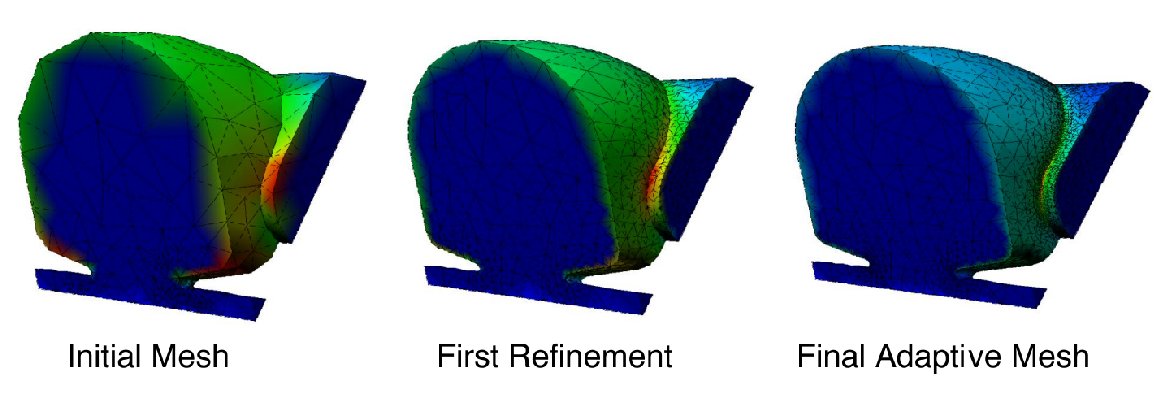
\epsfig{file=adapt-cavity.ps,width=10cm}
\caption{Adaptive analysis of a Trispal 4-petal accelerator cavity.}
\label{fig:trispalAdapt}
\end{center}
\end{figure}

\subsubsection{Metal Forming Simulation}

In 3D metal forming simulations, the workpiece undergoes large plastic
deformations that result in major changes in the domain geometry. The
meshes of the deforming parts typically need to be frequently modified
to continue the analysis due to large element distortions, mesh
discretization errors and/or geometric approximation errors. In these
cases, it is necessary to replace the deformed mesh with an improved
mesh that is consistent with the current geometry.  Procedures to
determine a new mesh size field considering each of these factors have
been developed and used in conjunction with local mesh modification
\cite{WaKo04}. The procedure includes functions to transfer history
dependent field variables as each mesh modification is performed
\cite{WaKo04}.

Figure~\ref{fig:forming} shows the set-up, initial mesh and final
adapted meshes for a steering link manufacturing problem solved using
the DEFORM-3D analysis engine \cite{Fl04} within a mesh
modification-based adaptive loop. A total stroke of 41.7mm is taken in
the simulation. The initial workpiece mesh consists 28,885
elements. The simulation is completed with 20 mesh modification steps
producing a final mesh with 102,249 elements.


\begin{figure}
\begin{center}
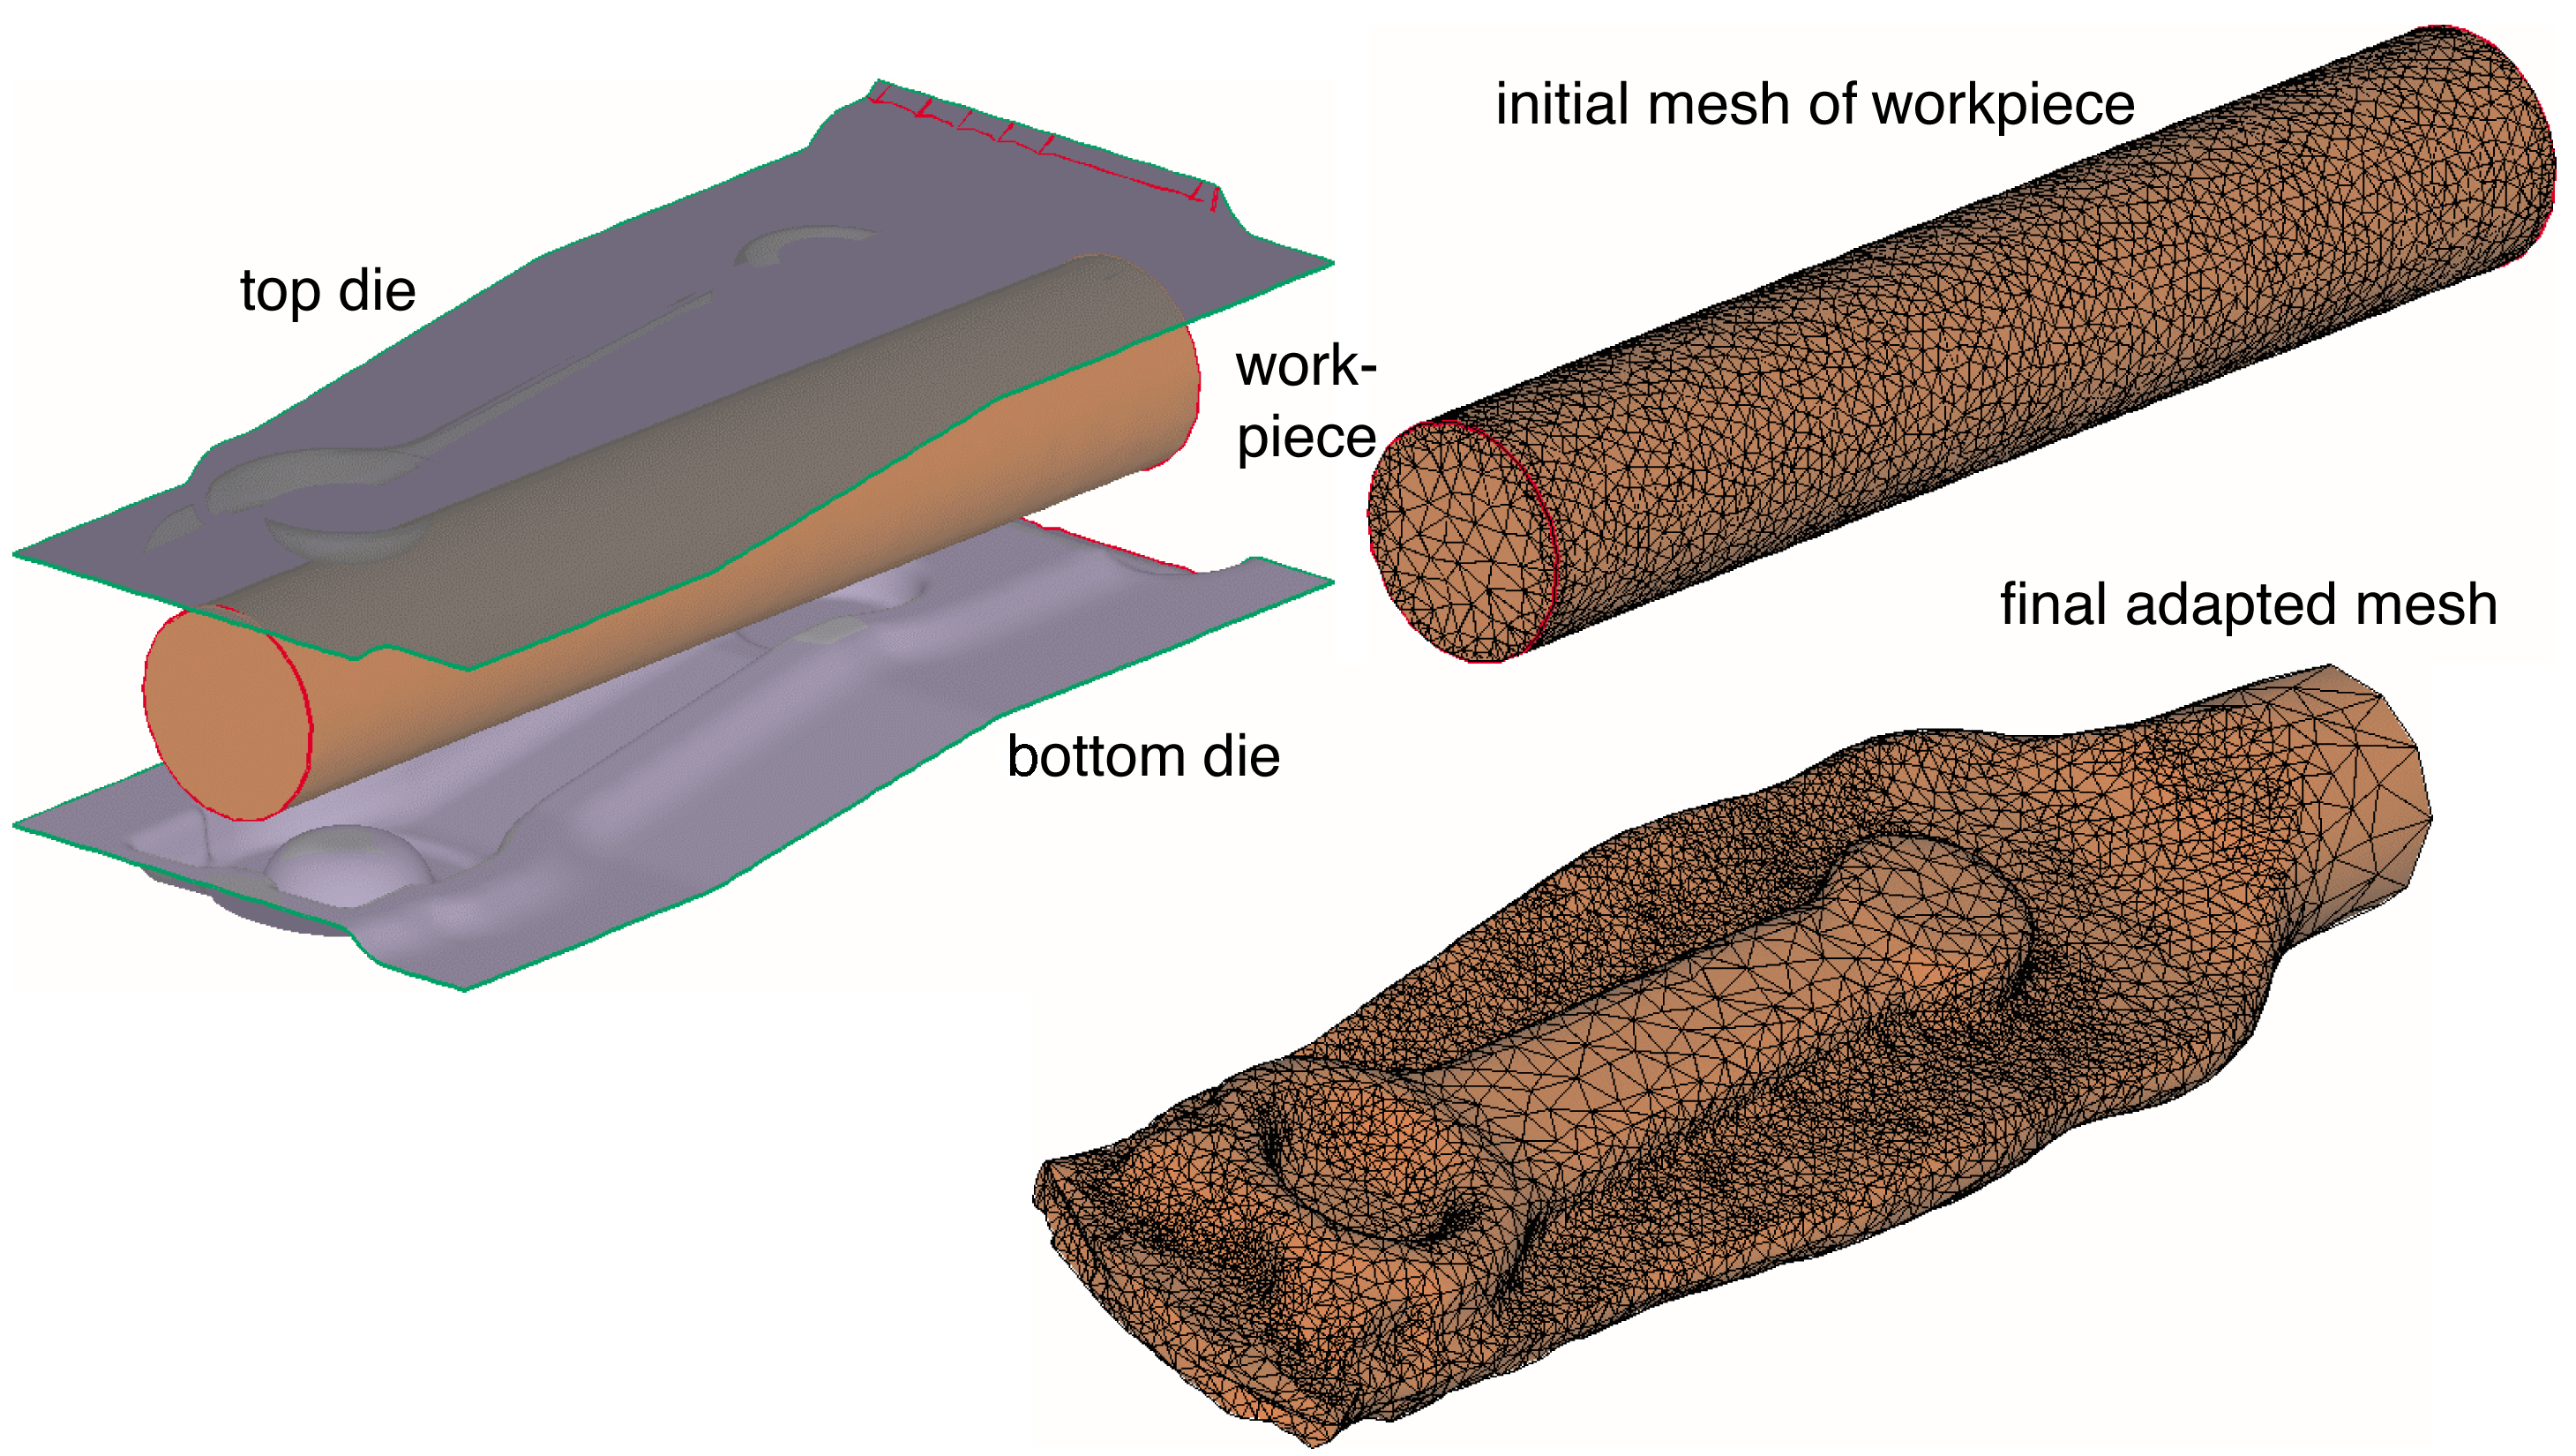
\epsfig{file=forming.ps,width=10cm}
\caption{Metal forming example.}
\label{fig:forming}
\end{center}
\end{figure}


